\documentclass[a4paper,10pt]{article}
\usepackage[brazilian]{babel}
\usepackage[left=2.5cm,right=2.5cm,top=3cm,bottom=2.5cm]{geometry}
\usepackage{mathtools}
\usepackage{amsthm}
\usepackage{amsmath}
%\usepackage{nccmath}
\usepackage{amssymb}
\usepackage{amsfonts}
\usepackage{physics}
%\usepackage{dsfont}
%\usepackage{mathrsfs}

\usepackage{titling}
\usepackage{indentfirst}

\usepackage{bm}
\usepackage[dvipsnames]{xcolor}
\usepackage{cancel}

\usepackage{xurl}
\usepackage[colorlinks=true]{hyperref}

\usepackage{float}
\usepackage{graphicx}
%\usepackage{tikz}
\usepackage{caption}
\usepackage{subcaption}

%%%%%%%%%%%%%%%%%%%%%%%%%%%%%%%%%%%%%%%%%%%%%%%%%%%

\newcommand{\eps}{\epsilon}
\newcommand{\vphi}{\varphi}
\newcommand{\cte}{\text{cte}}

\newcommand{\N}{\mathbb{N}}
\newcommand{\Z}{\mathbb{Z}}
\newcommand{\Q}{\mathbb{Q}}
\newcommand{\R}{\vb{R}}
\newcommand{\C}{\mathbb{C}}
\renewcommand{\S}{\hat{S}}
%\renewcommand{\H}{\s{H}}

\renewcommand{\a}{\vb{a}}
\newcommand{\nn}{\hat{n}}
\renewcommand{\d}{\dagger}
\newcommand{\up}{\uparrow}
\newcommand{\down}{\downarrow}

\newcommand{\0}{\vb{0}}
%\newcommand{\1}{\mathds{1}}
\newcommand{\E}{\vb{E}}
\newcommand{\B}{\vb{B}}
\renewcommand{\v}{\vb{v}}
\renewcommand{\r}{\vb{r}}
\renewcommand{\k}{\vb{k}}
\newcommand{\p}{\vb{p}}
\newcommand{\q}{\vb{q}}
\newcommand{\F}{\vb{F}}

\newcommand{\s}{\sigma}
%\newcommand{\prodint}[2]{\left\langle #1 , #2 \right\rangle}
\newcommand{\cc}[1]{\overline{#1}}
\newcommand{\Eval}[3]{\eval{\left( #1 \right)}_{#2}^{#3}}

\newcommand{\unit}[1]{\; \mathrm{#1}}

\newcommand{\n}{\medskip}
\newcommand{\e}{\quad \mathrm{e} \quad}
\newcommand{\ou}{\quad \mathrm{ou} \quad}
\newcommand{\virg}{\, , \;}
\newcommand{\ptodo}{\forall \,}
\renewcommand{\implies}{\; \Rightarrow \;}
%\newcommand{\eqname}[1]{\tag*{#1}} % Tag equation with name

\setlength{\droptitle}{-7em}

\theoremstyle{plain}
\newtheorem{theorem}{Teorema}[section]
%\newtheorem{defi}[theorem]{Definição}
\newtheorem{lemma}[theorem]{Lema}
%\newtheorem{corol}[theorem]{Corolário}
%\newtheorem{prop}[theorem]{Proposição}
%\newtheorem{example}{Exemplo}
%
%\newtheorem{inneraxiom}{Axioma}
%\newenvironment{axioma}[1]
%  {\renewcommand\theinneraxiom{#1}\inneraxiom}
%  {\endinneraxiom}
%
%\newtheorem{innerpostulado}{Postulado}
%\newenvironment{postulado}[1]
%  {\renewcommand\theinnerpostulado{#1}\innerpostulado}
%  {\endinnerpostulado}
%
%\newtheorem{innerexercise}{Exercício}
%\newenvironment{exercise}[1]
%  {\renewcommand\theinnerexercise{#1}\innerexercise}
%  {\endinnerexercise}
%
%\newtheorem{innerthm}{Teorema}
%\newenvironment{teorema}[1]
%  {\renewcommand\theinnerthm{#1}\innerthm}
%  {\endinnerthm}
%
\newtheorem{innerlema}{Lema}
\newenvironment{lema}[1]
  {\renewcommand\theinnerlema{#1}\innerlema}
  {\endinnerlema}
%
%\theoremstyle{remark}
%\newtheorem*{hint}{Dica}
%\newtheorem*{notation}{Notação}
%\newtheorem*{obs}{Observação}


\usepackage[shortlabels]{enumitem}

\title{\Huge{\textbf{Lista 1 - Estado Sólido 1}}}
\author{Mateus Marques}

\begin{document}

\maketitle

\section{}

(a)
\begin{itemize}
\item $\R$ é um vetor que pertence à rede de Bravais, ou seja, $\R = n_1 \a_1 + n_2 \a_2 + n_3 \a_3$, com $n_1,n_2,n_3$
inteiros e $\a_1,\a_2,\a_3$ os vetores primitivos da rede de Bravais.

\item $\G$ é vetor da rede recíproca, que satisfaz $e^{i \G \vdot \R} = 1$, $\ptodo \R \in$ rede de Bravais.

\item $V_{\G}$ são as componentes da transformada discreta de Fourier do potencial periódico
$$
V(\r) = \sum_{\G} V_{\G} e^{i \G \vdot \R}.
$$

\item $\k$ é um vetor qualquer do espaço recíproco. Mas devido à periodicidade da rede recíproca, podemos tomar $\k \in$ Zona de Brillouin.

\end{itemize}


(b) Um ``mesmo ponto'' de diferentes células unitárias diferem-se apenas por vetores $\R \in$ Rede de Bravais. Assim, dadas duas células unitárias $\Omega$ e $\Omega'$, o ``mesmo ponto'' na célula $C'$ é da forma $\r' = \r + \R$. Temos então
$$
\psi_\k(\r') = \psi_\k(\r+\R) = e^{i \k \vdot (\r+\R)} \underbrace{u_\k(\r+\R)}_{=u_\k(\r)} =
e^{i \k \vdot \R} \qty[e^{i\k\vdot\r} u_\k(\r)] = e^{i\k\vdot\R} \psi_\k(\r).
$$

Portanto
$$
\abs{\psi_\k(\r')}^2 = \abs{\psi_\k(\r)}^2,
$$
ou seja, a probabilidade de encontrar um elétron (no estado $\k$) no ponto $\r'$ é a mesma de encontrar no ponto $\r$.


\pagebreak

\section{}

\begin{enumerate}[(a)]
\item Falso para o espaço recíproco!

Para o espaço direto é indiferente a escolha da origem, pois sempre podemos redefinir os vetores da base, mantendo os vetores primitivos da rede de Bravais.

Para o espaço recíproco importa a escolha da origem devido ao ponto $\Gamma$ (que é o de mais alta simetria) e também porque a energia $\eps(\k)$ depende de $\k$. Por exemplo, no caso de elétrons livres $\eps(\k) = \hbar^2 \k^2 / 2m$. Se deslocarmos a origem do espaço recíproco por um vetor $\vb{Q}$, isso faz com que os elétrons certo momento $\k$ mudem de energia $\eps(\k) = \hbar^2 \k^2 / 2m$ para $\eps(\k+\vb{Q}) = \hbar^2 (\k+\vb{Q})^2 / 2m$.

\item Falso!

Existem infinitas escolhas diferentes de células primitivas tanto para uma dada rede de Bravais. Assim, tanto para o espaço direto quanto para o espaço recíproco a escolha de montagem de células primitivas \textbf{não é única}.

\begin{figure}[H]
\centering
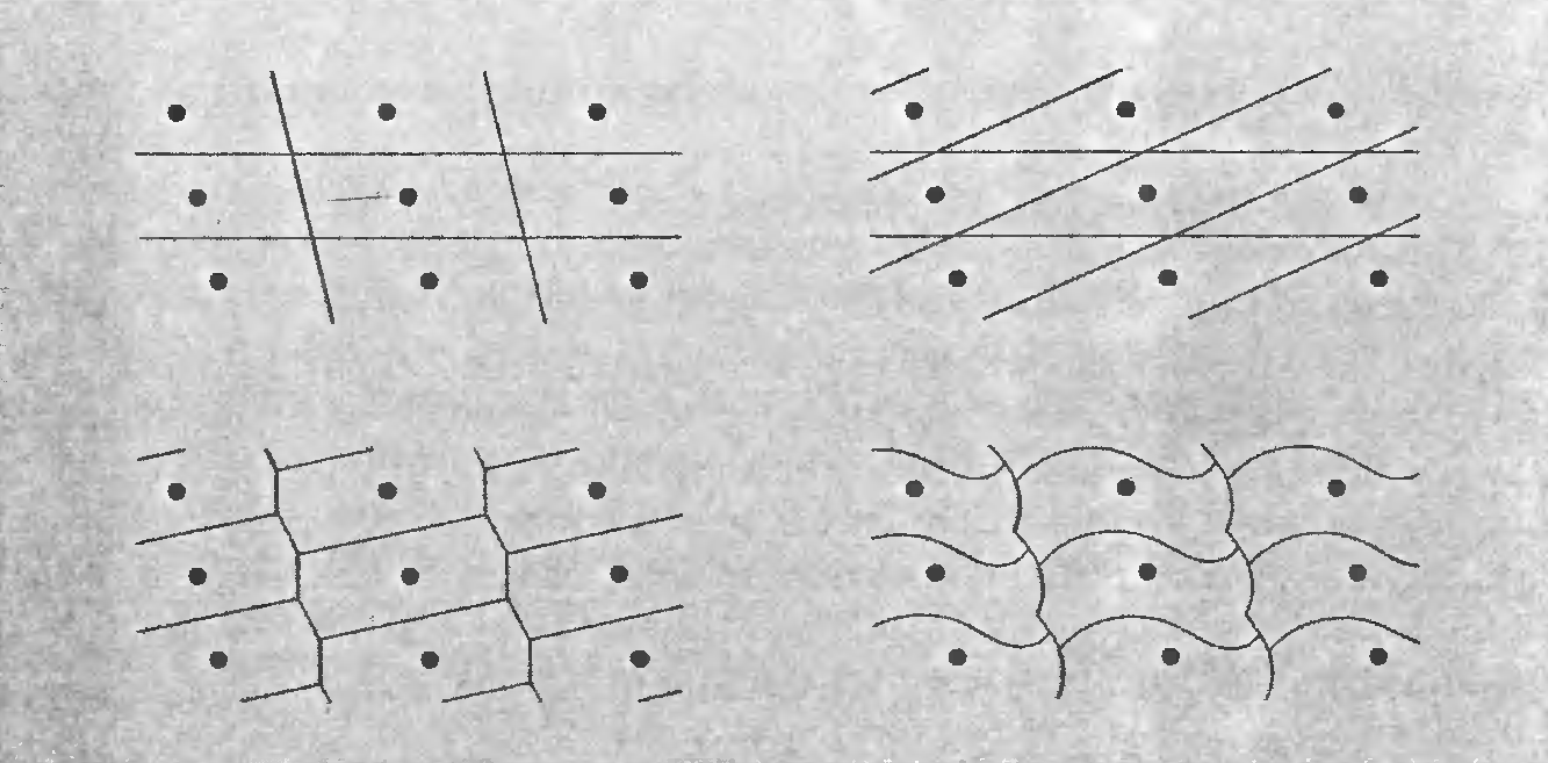
\includegraphics[width=\linewidth]{fig/primitive_cells.png}
\caption{Diferentes possíveis escolhas de célula primitiva para uma única rede de Bravais. Figura 4.10 do Ashcroft \& Mermin.}
\label{fig:primitive_cells}
\end{figure}


\item Verdade!

Lendo o Ashcroft \& Mermin (Capítulo 8), aprendemos que \textit{o número de vetores de onda $\k$ permitidos em uma célula primitiva da rede recíproca é igual ao número de sítios no cristal.} Lembre-se também que cada estado $\k$ acomoda 2 elétrons devido ao spin.

A Zona de Brillouin é a célula Wigner-Seitz da rede recíproca, portanto ela se trata de uma célula primitiva da rede recíproca e acomoda $2 N$ elétrons. Se o cristal tem $N$ sítios e 2 elétrons por célula unitária, então o sistema possui um total de $2N$ elétrons, que é exatamente o número de elétrons que a Zona de Brillouin acomoda. Finalmente, concluimos que nesse caso todos os pontos da primeira Zona de Brillouin estarão preenchidos.

\item Falso!

Na página seguinte mostrarei o cálculo da DOS nos casos 1D, 2D e 3D que eu escrevi numa lista da disciplina de Estado Sólido 2, que cursei semestre passado com o Prof. Eric Andrade. No cálculo eu utilizo a convenção $\hbar = 1$.

\pagebreak

A dispersão de elétrons livres é $E(\k) = \frac{k^2}{2m}$, com a substituição $\sum_{\k} \to \frac{V_d}{(2\pi)^d} \int \dd[d]{k}$,
$$
\rho_d(\eps) = \sum_{\k, \s} \delta(\eps - E(\k)) =
\frac{2V_d}{(2\pi)^d} \int \delta\qty(\eps - \frac{k^2}{2m}) \dd[d]{k} =
\frac{2V_d}{(2\pi)^d} \int \dd{\Omega_d} \int_0^\infty \delta\qty(\eps - \frac{k^2}{2m}) k^{d-1} \dd{k},
$$
onde $\Theta_d = \int \dd{\Omega_d}$ é o ângulo sólido de acordo com a dimensão $d$, sendo $\Theta_1 = 2, \Theta_2 = 2\pi$ e $\Theta_3 = 4\pi$.

Vale a seguinte propriedade da função $\delta$ de Dirac:
$$
\int_{D} f(x) \delta(g(x)) \dd{x} =
\sum_{\substack{g(a)=0 \\ a \in D}} \frac{1}{\abs{g'(a)}} \int_{-\infty}^{\infty} f(x) \delta(x-a) \dd{x}=
\sum_{\substack{g(a)=0 \\ a \in D}} \frac{1}{\abs{g'(a)}} \, f(a).
$$
onde a soma é sobre todos os zeros $a \in D$ da função $g(x)$ dentro do domínio de integração $D$.

Definindo $g(k) = \eps - \frac{k^2}{2m}$, temos $\abs{g'(k)} = \abs{k} / m$ e sua única raiz no domínio $D = (0, +\infty)$ é $k = \sqrt{2m \eps}$. Portanto
$$
\rho_d(\eps) = \frac{2V_d}{(2\pi)^d} \Theta_d \, \frac{m}{\sqrt{2m\eps}}
\qty(\sqrt{2m \eps})^{d-1} \implies
\boxed{ \rho_d(\eps) = \frac{2 m V_d \Theta_d}{(2\pi)^d} \, (2m\eps)^{\frac{d}{2}-1}. }
$$

Substituindo explicitamente as dimensões $d = 1, 2$ e $3$:
\begin{itemize}
\item $d = 1$, $V_1 = L$, $\Theta_1 = 2$:
$$
\boxed{\rho_1(\eps) = \frac{2 m L}{\pi} \, \frac{1}{\sqrt{2m\eps}}.}
$$
\item $d = 2$, $V_2 = A$, $\Theta_2 = 2\pi$:
$$
\boxed{\rho_2(\eps) = \frac{m A}{\pi}.}
$$
\item $d = 3$, $V_3 = V$, $\Theta_3 = 4\pi$:
$$
\boxed{\rho_3(\eps) = \frac{m V}{\pi^2} \sqrt{2m\eps}.}
$$
\end{itemize}

\begin{figure}[H]
\centering
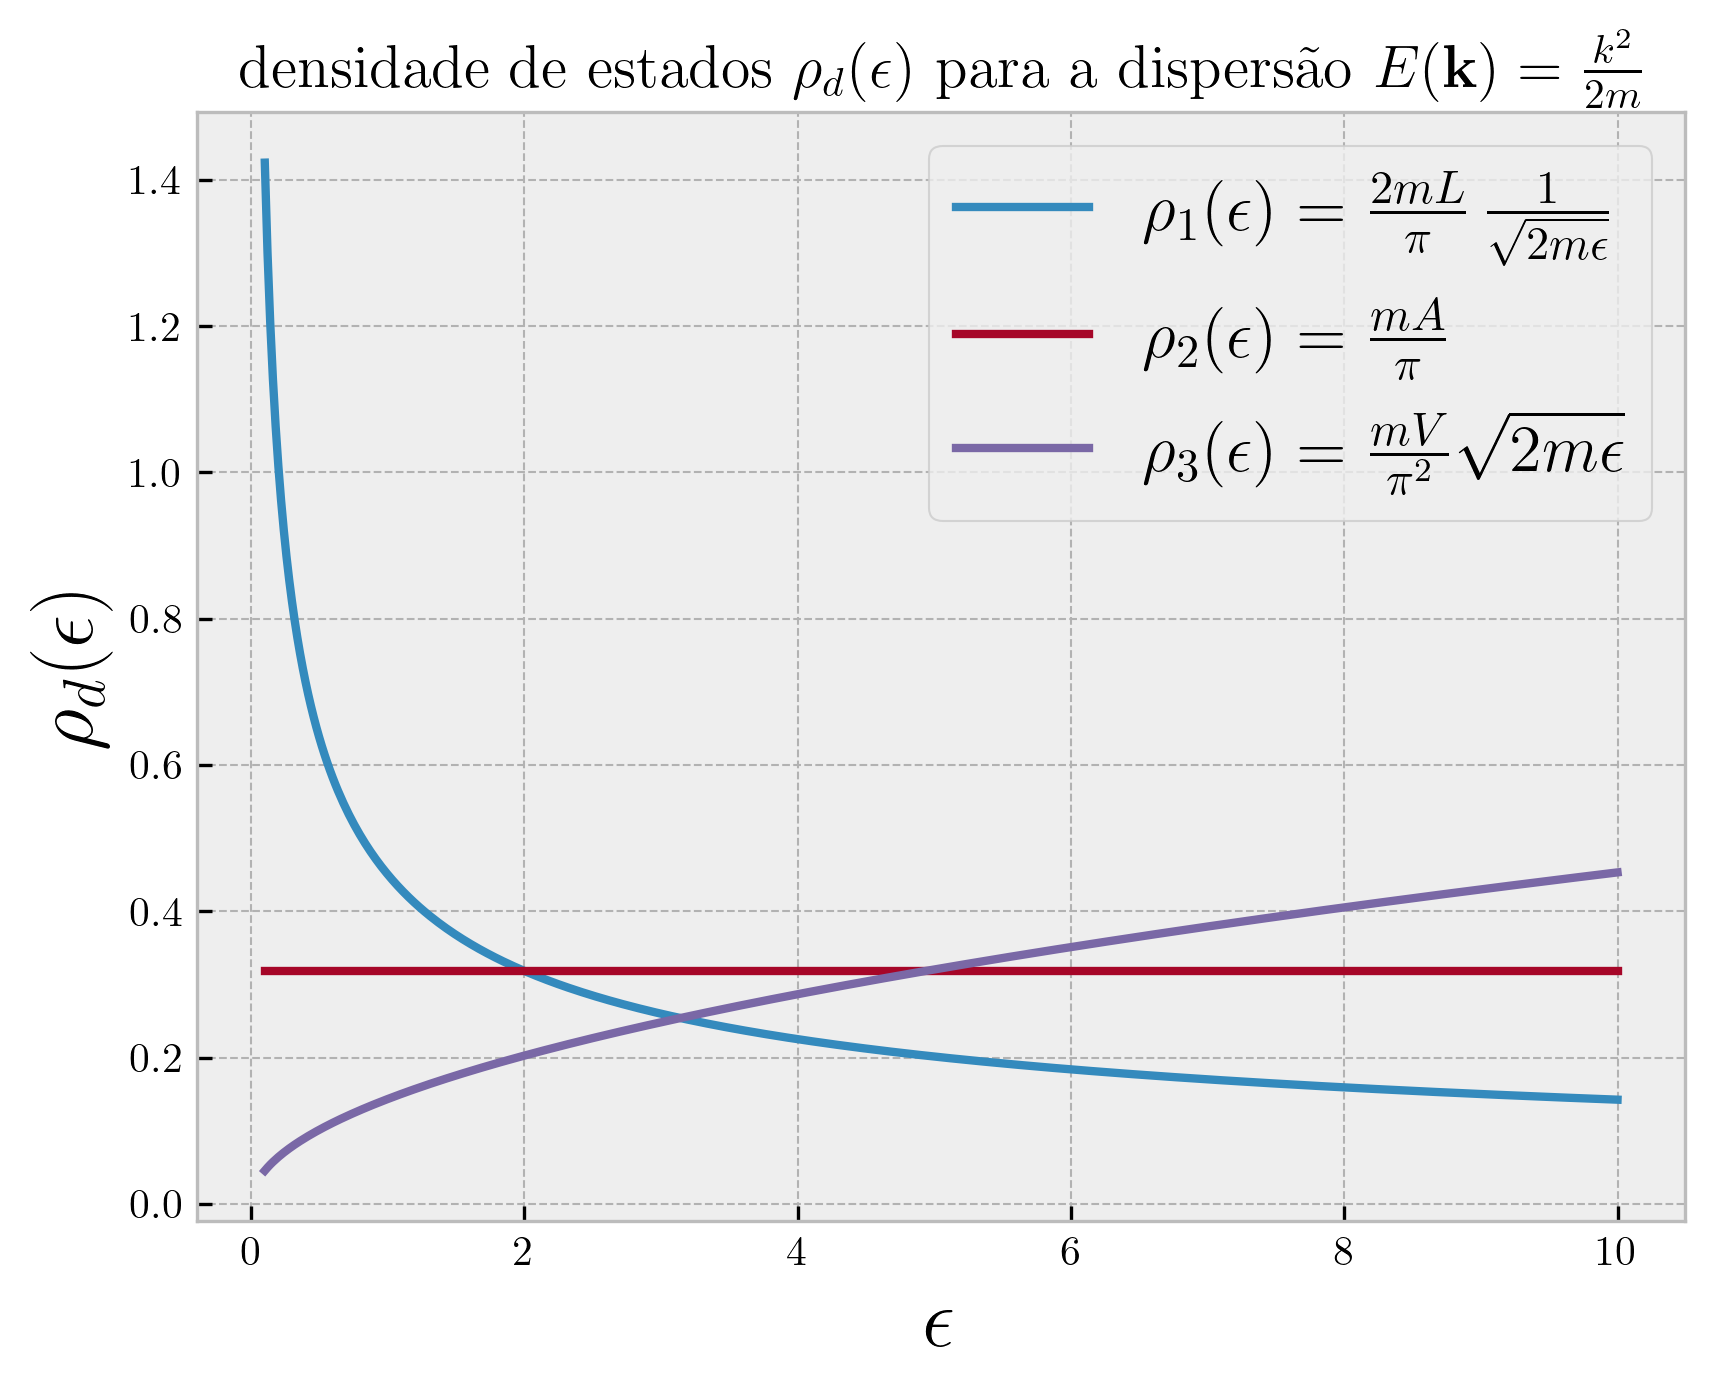
\includegraphics[width=0.79\textwidth]{fig/dos-k2.png}
\caption{Densidade de estados $\rho_d(\eps)$ para as dimensões $d = 1, 2$ e $3$. Parâmetros: $m = L = A = V = 1$.}
\label{fig:dosk2}
\end{figure}

\end{enumerate}



\pagebreak

\section{}

(a) Os vetores primitivos convencionais da rede quadrada são $\a_1 = a \vu{x}$, $\a_2 = a \vu{y}$ e $\a_3 = \vu{z}$. Sendo $\Omega = \abs{\a_1 \vdot (\a_2 \cross \a_2)} = a^2$, podemos calcular os vetores da rede recíproca como
$$
\b_1 = \frac{2\pi}{\Omega} (\a_2 \times \a_3) = \frac{2\pi}{a} \vu{x} \e \b_2 = \frac{2\pi}{\Omega}(\a_3 \times \a_1) = \frac{2\pi}{a} \vu{y}.
$$

A zona de Brillouin e os pontos de alta simetria estão exibidos na Figura \ref{fig:square_lattice_bz}:
\begin{figure}[H]
\centering
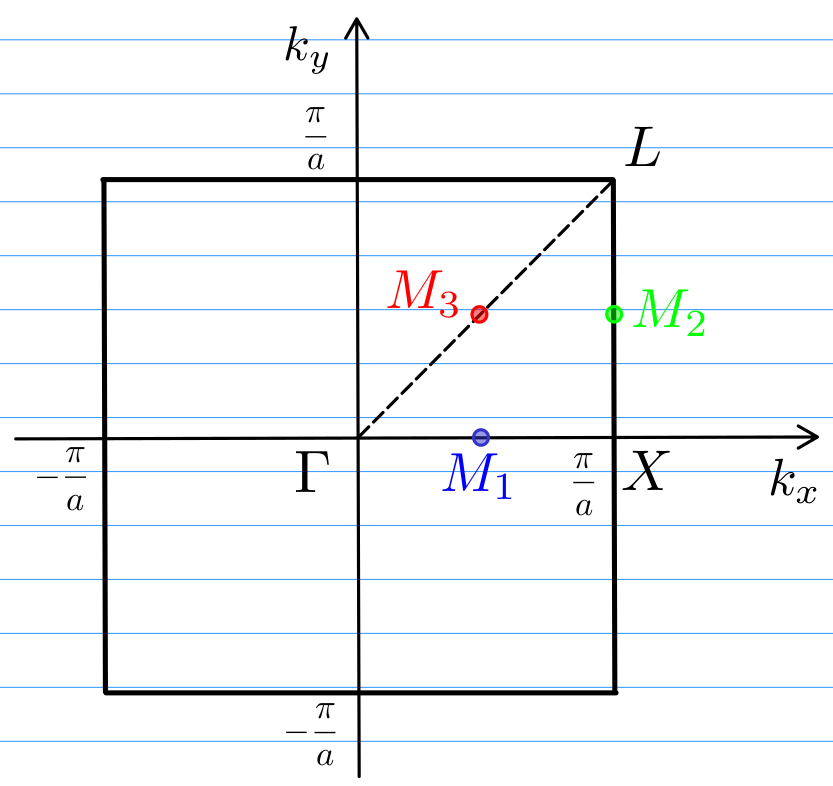
\includegraphics[width=0.4\linewidth]{fig/square_lattice_bz.png}
\caption{Zona de Brillouin da rede quadrada. $\Gamma$, $L$ e $X$ são os pontos de simetria importantes. Os pontos $M_1$, $M_2$ e $M_3$ são os pontos medianos em cada linha de alta simetria.}
\label{fig:square_lattice_bz}
\end{figure}

\n

(b) Olhando para a Figura \ref{fig:square_lattice_bz}, é fácil identificar as coordenadas $(k_x, k_y)$ de todos os pontos:
$$
\Gamma = \qty(0, 0), \quad
X = \qty(\frac{\pi}{a}, 0), \quad
L = \qty(\frac{\pi}{a}, \frac{\pi}{a}), \quad
M_1 = \qty(\frac{\pi}{2a}, 0), \quad
M_2 = \qty(\frac{\pi}{a}, \frac{\pi}{2a}), \quad
M_3 = \qty(\frac{\pi}{2a}, \frac{\pi}{2a}).
$$

Pela relação de dispersão $\displaystyle{\eps(k_x, k_y) = \frac{\hbar^2 (k_x^2 + k_y^2)}{2m_e}}$ e usando a unidade $\displaystyle{\mathcal{E} = \frac{\hbar^2 \pi^2}{2 m_e a^2}}$, obtemos que
$$
\eps(\Gamma) = 0, \quad
\eps(X) = \frac{\hbar^2 \pi^2}{2 m_e a^2} = \mathcal{E}, \quad
\eps(L) = \frac{\hbar^2 \pi^2}{m_e a^2} = 2 \mathcal{E},
$$
$$
\eps(M_1) = \frac{\hbar^2 \pi^2}{8 m_e a^2} = \frac{\mathcal{E}}{4}, \quad
\eps(M_2) = \frac{5\hbar^2 \pi^2}{8 m_e a^2} = \frac{5\mathcal{E}}{4}, \quad
\eps(M_3) = \frac{\hbar^2 \pi^2}{4 m_e a^2} = \frac{\mathcal{E}}{2}.
$$

\begin{figure}[H]
\centering
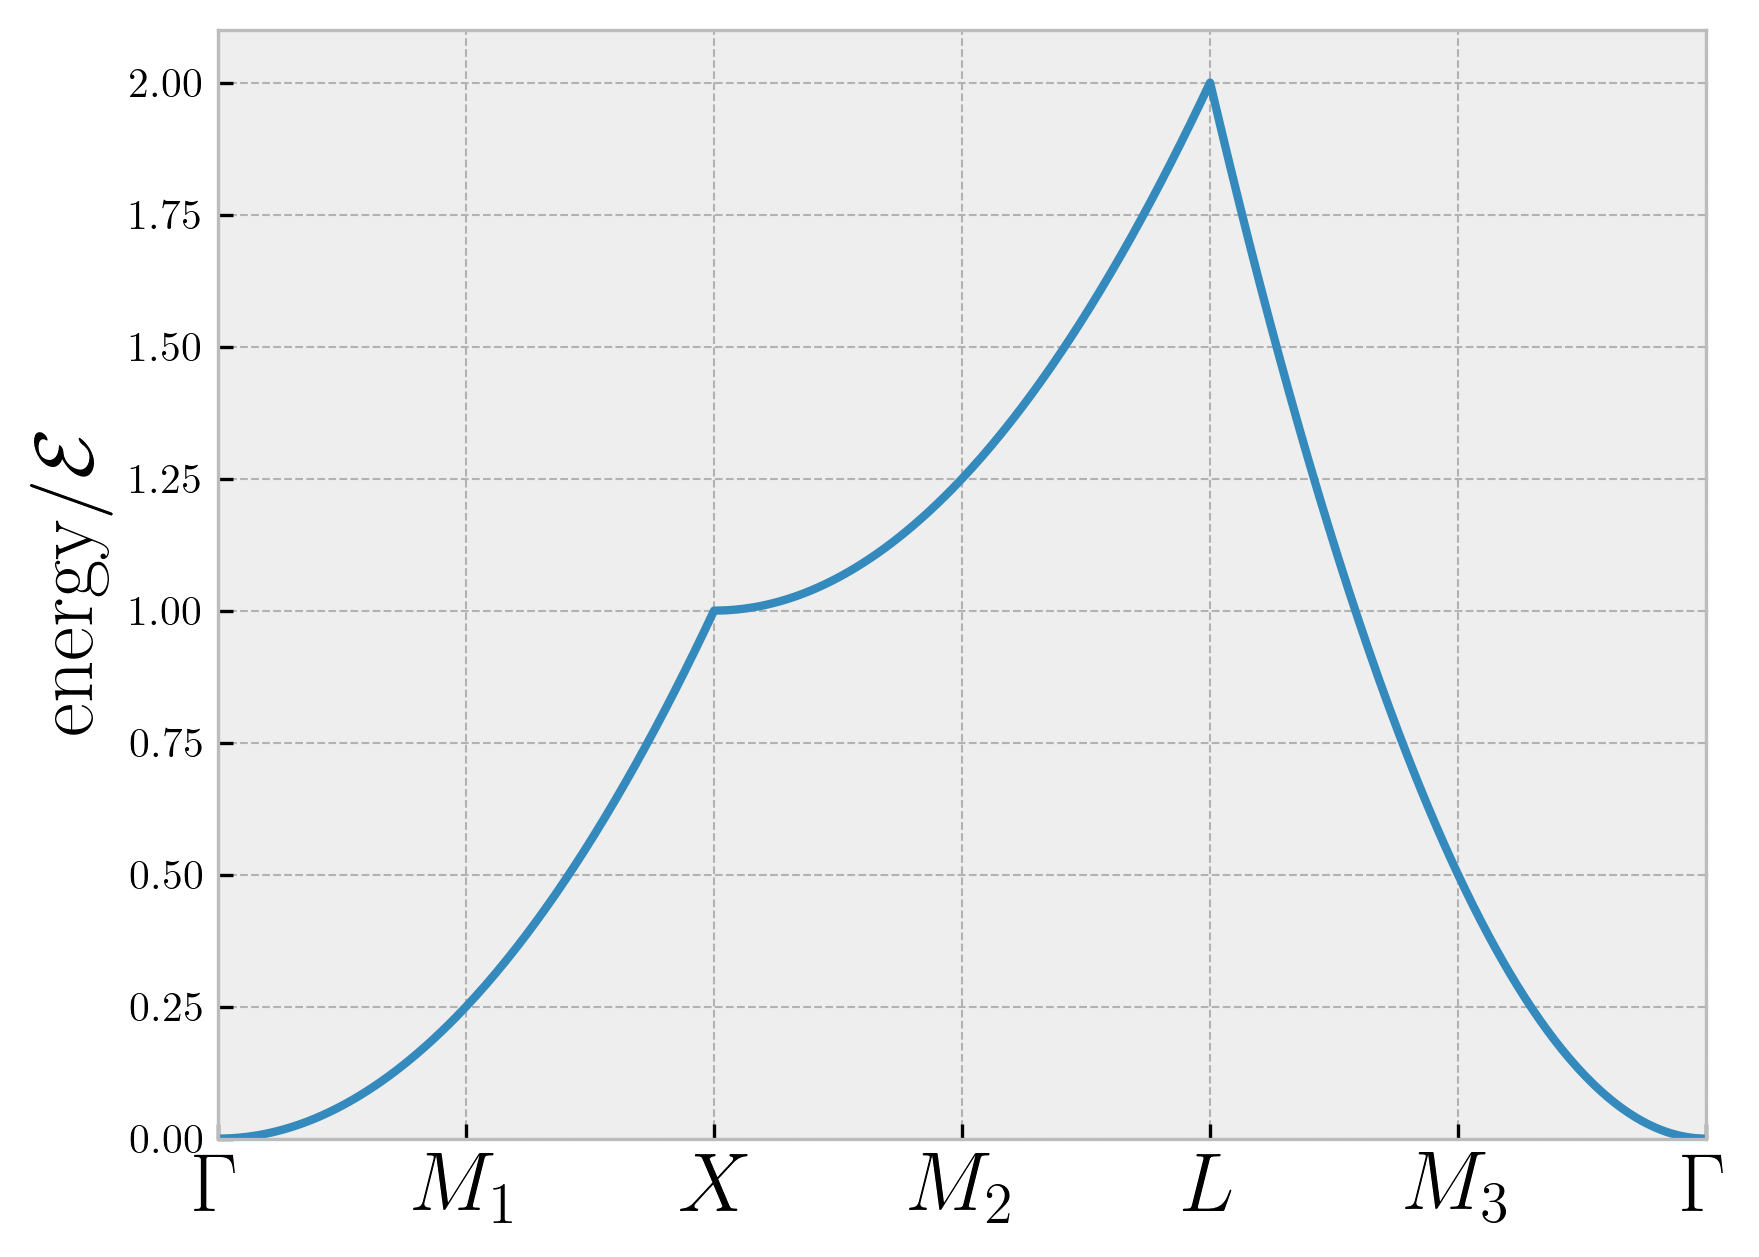
\includegraphics[width=0.5\linewidth]{fig/band_struct_square_free.png}
\caption{Primeira banda para elétrons livres na rede quadrada 2D graficada no Python.}
\label{fig:band_struct_square_free}
\end{figure}

(c) Na Figura \ref{fig:squarebz} deslocamos as 2\textsuperscript{\underline{a}} e 3\textsuperscript{\underline{a}} zonas de Brillouin para a primeira.

\begin{figure}[H]
\centering
\begin{subfigure}{.4\textwidth}
  \centering
  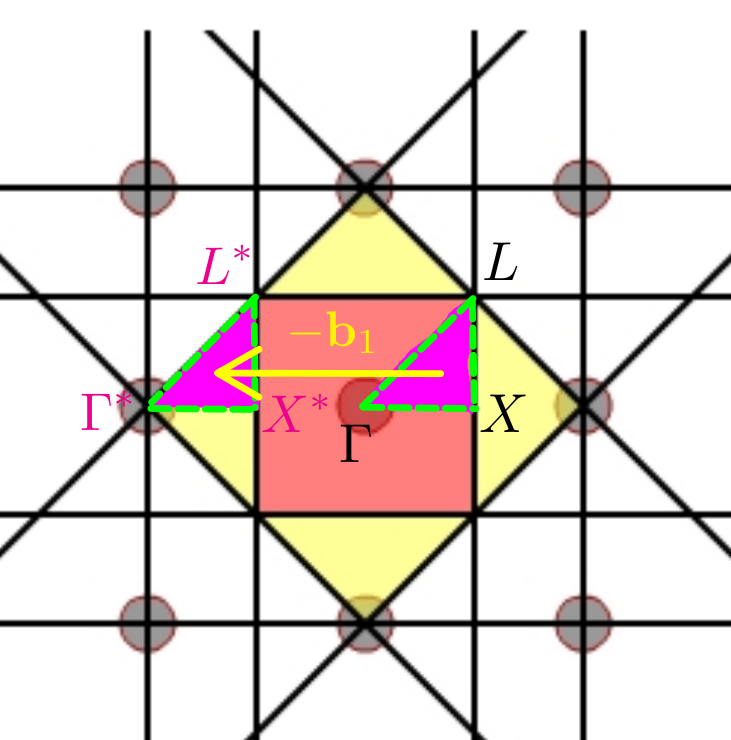
\includegraphics[width=\linewidth]{fig/squarebz-2nd.png}
\end{subfigure}
\quad \quad
\begin{subfigure}{.4\textwidth}
  \centering
  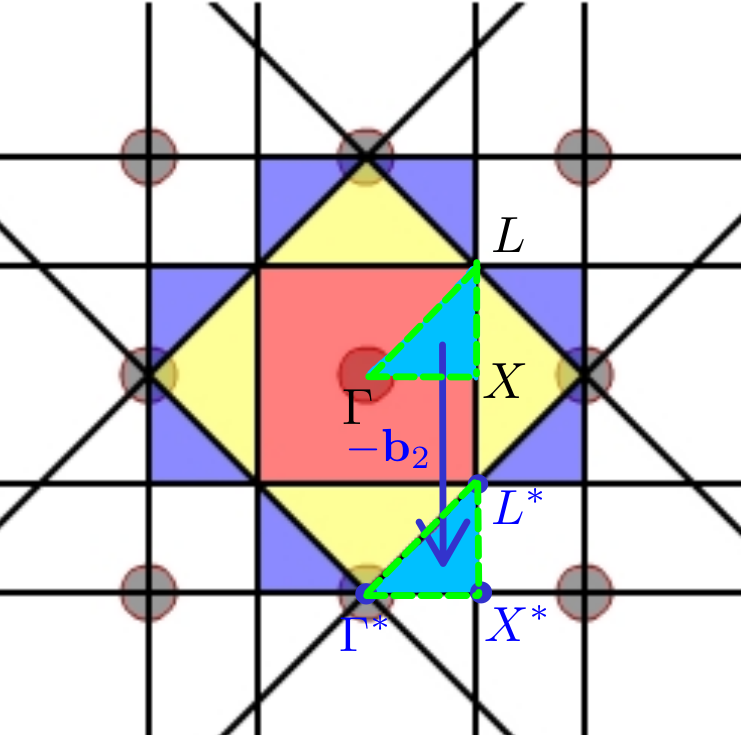
\includegraphics[width=\linewidth]{fig/squarebz-3rd.png}
\end{subfigure}
\caption{Deslocamento da 2\textsuperscript{\underline{a}} e 3\textsuperscript{\underline{a}} zonas de Brillouin, pelos vetores de rede $-\b_1$ e $-\b_2$, respectivamente. Os pontos $\Gamma, X$ e $L$ são deslocados para $\Gamma^*, X^*$ e $L^*$.}
\label{fig:squarebz}
\end{figure}

\n\n

Graficando no Python a energia pelo caminho dos pontos deslocados $\Gamma^* \to X^* \to L^* \to \Gamma^*$ para as 2\textsuperscript{\underline{a}} e 3\textsuperscript{\underline{a}} zonas de Brillouin, obtemos a segunda (vermelha) e terceira (violeta) bandas de energia, exibidas na Figura \ref{fig:band_struct_square_free-123}.
\begin{figure}[H]
\centering
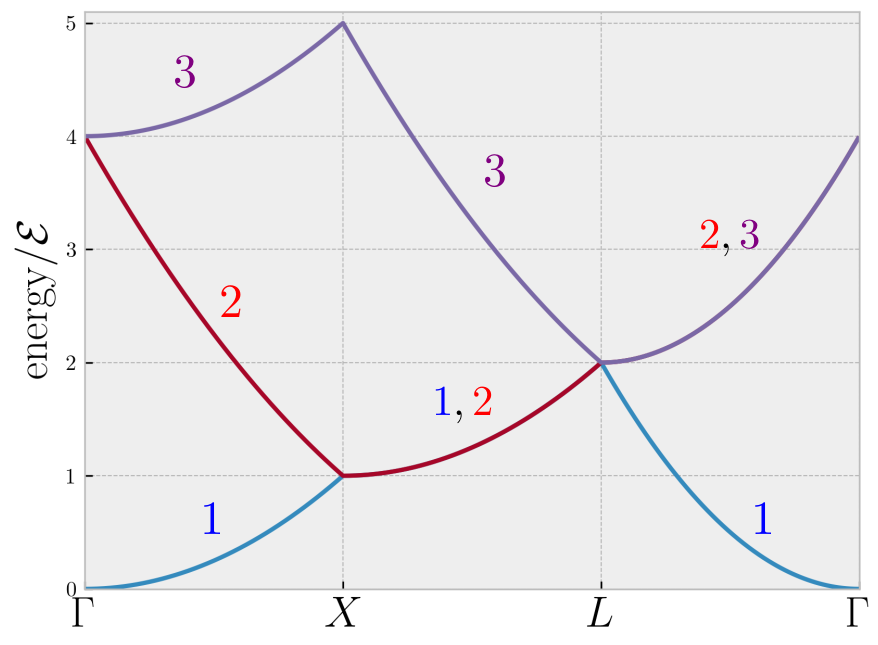
\includegraphics[width=0.7\linewidth]{fig/band_struct_square_free-123-labels.png}
\caption{Três primeiras bandas (azul, vermelha e violeta, respectivamente) para elétrons livres na rede quadrada 2D.}
\label{fig:band_struct_square_free-123}
\end{figure}

\n

Identificamos as degenerescências em energia na região da Figura \ref{fig:band_struct_square_free-123} onde duas bandas coincidem. Assim, temos uma degenerescência na linha $X \to L$ entre as bandas 1 e 2 e outra degenerescência na linha $L \to \Gamma$ entre as bandas 2 e 3.

\pagebreak

\section{}

(a)

\begin{figure}[H]
\centering
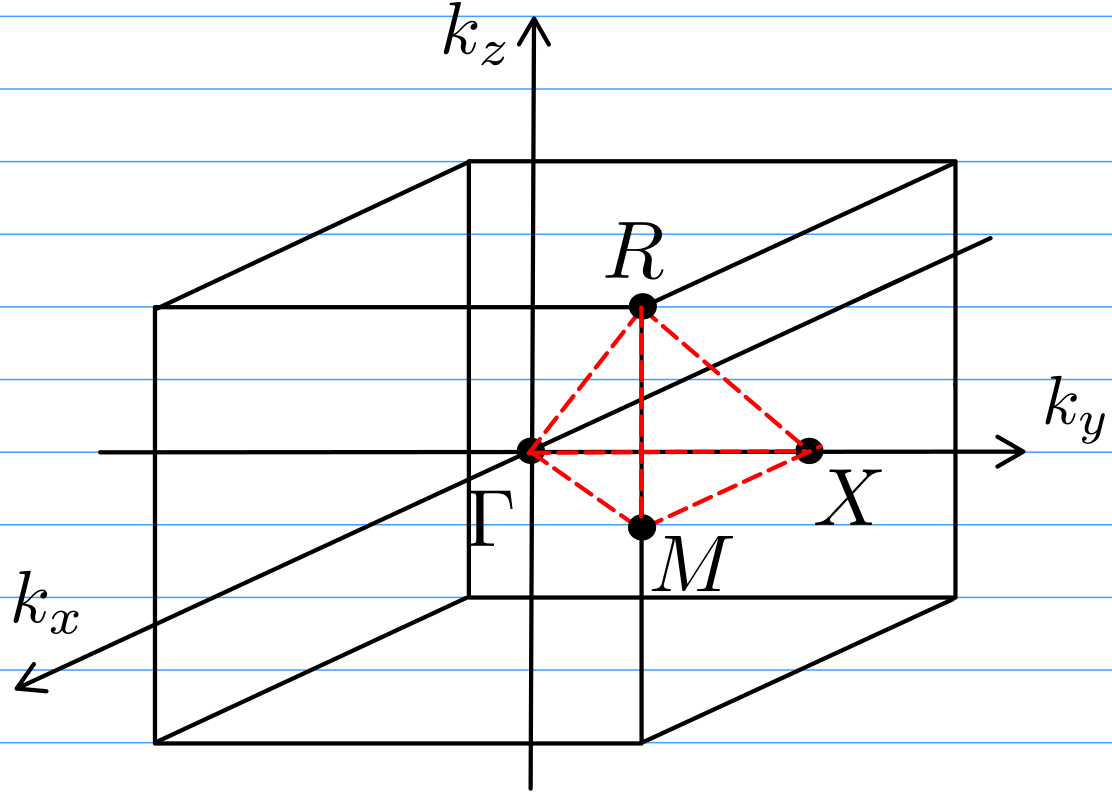
\includegraphics[width=0.4\linewidth]{fig/cubicbz.png}
\caption{Zona de Brillouin da rede cúbica, pontos e linhas de alta simetria.}
\label{fig:cubicbz}
\end{figure}

Reaproveitando o script em Python que usei na Figura \ref{fig:band_struct_square_free}, utilizei ele para graficar a estrutura de bandas tight-binding $\eps(\k) = -\eps_0 (\cos k_x a + \cos k_y a + \cos k_z a)$ para a rede cúbica na Figura \ref{fig:band_struct_cubic_free} a seguir.
\begin{figure}[H]
\centering
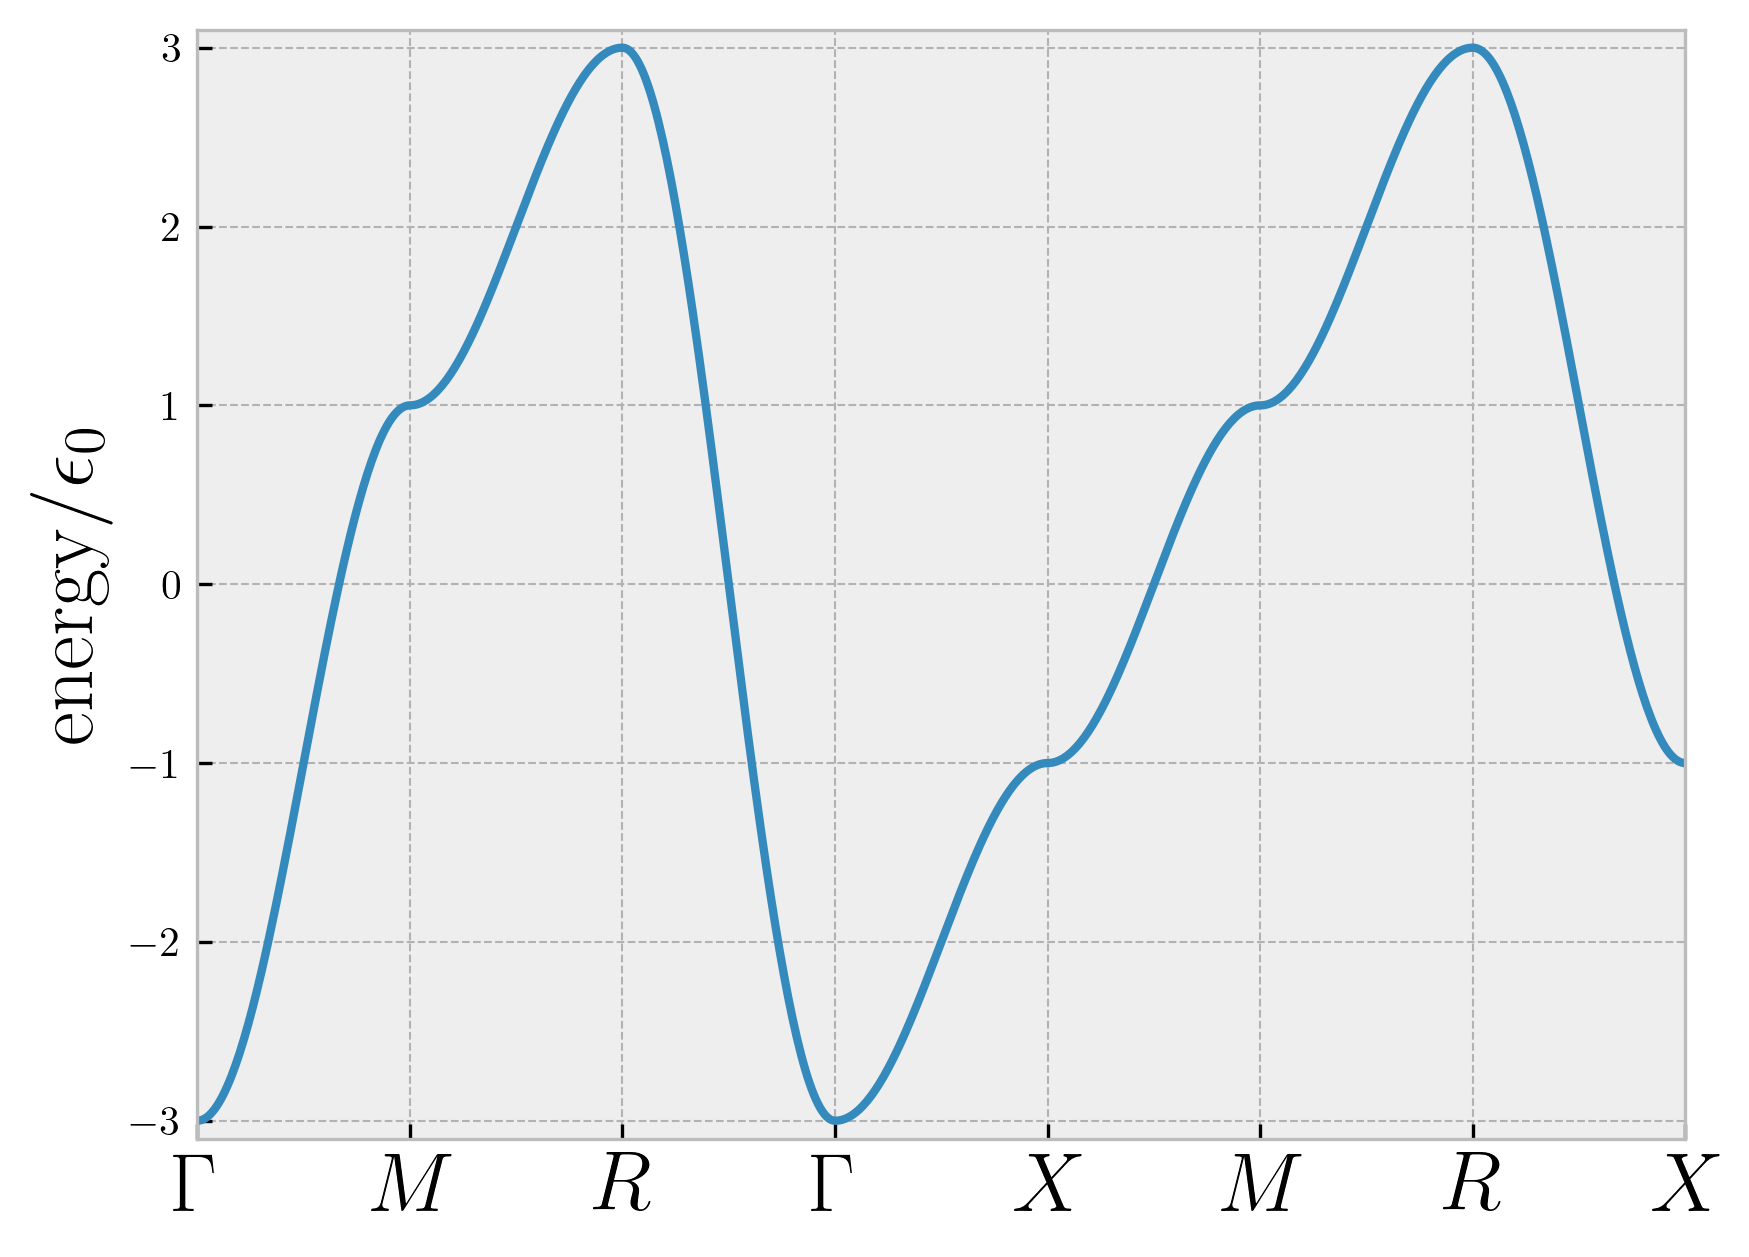
\includegraphics[width=0.5\linewidth]{fig/band_struct_cubic_free.png}
\caption{Estrutura de bandas tight-binding para a rede cúbica.}
\label{fig:band_struct_cubic_free}
\end{figure}

(b) O tensor massa efetiva é definido por
$$
\mathcal{M}^{-1}_{ij} = \frac{1}{\hbar^2} \pdv{\eps}{k_i}{k_j}.
$$

Para uma mesma direção temos
$$
\mathcal{M}_{xx}^{-1} = \frac{1}{\hbar^2} \pdv[2]{\eps}{k_x} = \frac{\eps_0 a^2}{\hbar^2} \cos(k_x a).
$$

Analogamente, temos $\mathcal{M}_{yy}^{-1} = \frac{\eps_0 a^2}{\hbar^2} \cos(k_y a)$ e $\mathcal{M}_{zz}^{-1} = \frac{\eps_0 a^2}{\hbar^2} \cos(k_z a)$.

\n\n

Para direções diferentes, é fácil ver que
$$
\mathcal{M}_{xy}^{-1} = \mathcal{M}_{xz}^{-1} = \mathcal{M}_{yz}^{-1} = 0.
$$

De maneira que
$$
\mathcal{M}(\k) =
\frac{\hbar^2}{\eps_0 a^2}
\begin{pmatrix}
\frac{1}{\cos(k_x a)} & 0 & 0 \\
0 & \frac{1}{\cos(k_y a)} & 0 \\
0 & 0 & \frac{1}{\cos(k_z a)} \\
\end{pmatrix}.
$$

Em especial, nos pontos $\Gamma$ e $R$:
$$
\mathcal{M}(\Gamma) =
\frac{\hbar^2}{\eps_0 a^2}
\begin{pmatrix}
1 & 0 & 0 \\
0 & 1 & 0 \\
0 & 0 & 1 \\
\end{pmatrix},
$$
$$
\mathcal{M}(R) =
\frac{\hbar^2}{\eps_0 a^2}
\begin{pmatrix}
-1 & 0 & 0 \\
0 & -1 & 0 \\
0 & 0 & -1 \\
\end{pmatrix}.
$$

(c) Notamos então que há comportamento de elétron (massa positiva) no ponto $\Gamma$ (de mais baixa energia $-3\eps_0$) e comportamento de buraco (massa negativa) no ponto $R$ (de mais alta energia $+3\eps_0$). Pela Figura \ref{fig:band_struct_cubic_free} é possível ver que a energia cresce mais rapidamente na direção $\Gamma \to R$ do que na direção $\Gamma \to X$. Isso significa que na direção $\Gamma \to R$ os elétrons são possuem uma massa efetiva mais leve.

\end{document}
